\section{Results and Discussion}
\label{sec:results}
We first provide results of the case study before commenting on the general application of conflict-measuring methods across multi-objective systems.

\subsection{Case Study Results}
We parameterized and solved the multi-objective model (\eqref{eqn:objFire}-\eqref{eqn:constraintNonNeg}) for each of the climate scenarios, generating three efficient frontiers: $Z_{\text{None}}$, $Z_{E45}$, and $Z_{E85}$ for the None, Ensemble RCP 4.5, and Ensemble RCP 8.5 scenarios, respectively. Figure \ref{fig:frontiersAll} shows the frontiers in their 3-dimensional objective spaces while Figure \ref{fig:frontiersPCPlot} provides a parallel coordinates view of the frontiers; their summary details are listed in Table \ref{tab:frontiersSummary}.

\begin{table}[]
\centering
\caption[Summary of efficient frontiers]{Summary of the performance of the efficient frontiers for each climate change scenario.}
\label{tab:frontiersSummary}
\begin{tabular}{lllll}
\multicolumn{2}{l|}{}                                                  & \textbf{None} & \textbf{E45} & \textbf{E85} \\ \hline
\multirow{3}{*}{\textbf{Fire hazard}}       & \multicolumn{1}{l|}{min} & 21321.21      & 23219.82     & 23268.02     \\
                                            & \multicolumn{1}{l|}{max} & 21933.29      & 23973.79     & 23724.98     \\
                                            & \multicolumn{1}{l|}{avg} & 21406.26      & 23324.41     & 23369.57     \\ \hline
\multirow{3}{*}{\textbf{NSO habitat}}       & \multicolumn{1}{l|}{min} & 2532.33       & 2412.18      & 2171.10      \\
                                            & \multicolumn{1}{l|}{max} & 2540.05       & 2477.18      & 2481.01      \\
                                            & \multicolumn{1}{l|}{avg} & 2536.31       & 2447.92      & 2421.99      \\ \hline
\multirow{3}{*}{\textbf{Sediment delivery}} & \multicolumn{1}{l|}{min} & 0             & 0            & 0            \\
                                            & \multicolumn{1}{l|}{max} & 24.57         & 63.43        & 69.68        \\
                                            & \multicolumn{1}{l|}{avg} & 10.25         & 27.98        & 31.19        \\ \hline
\multicolumn{2}{l}{\textbf{Number of solutions}}                       & 51            & 701          & 1083        
\end{tabular}
\end{table}


\begin{figure}[ht!]
  \subfloat[None]{%
    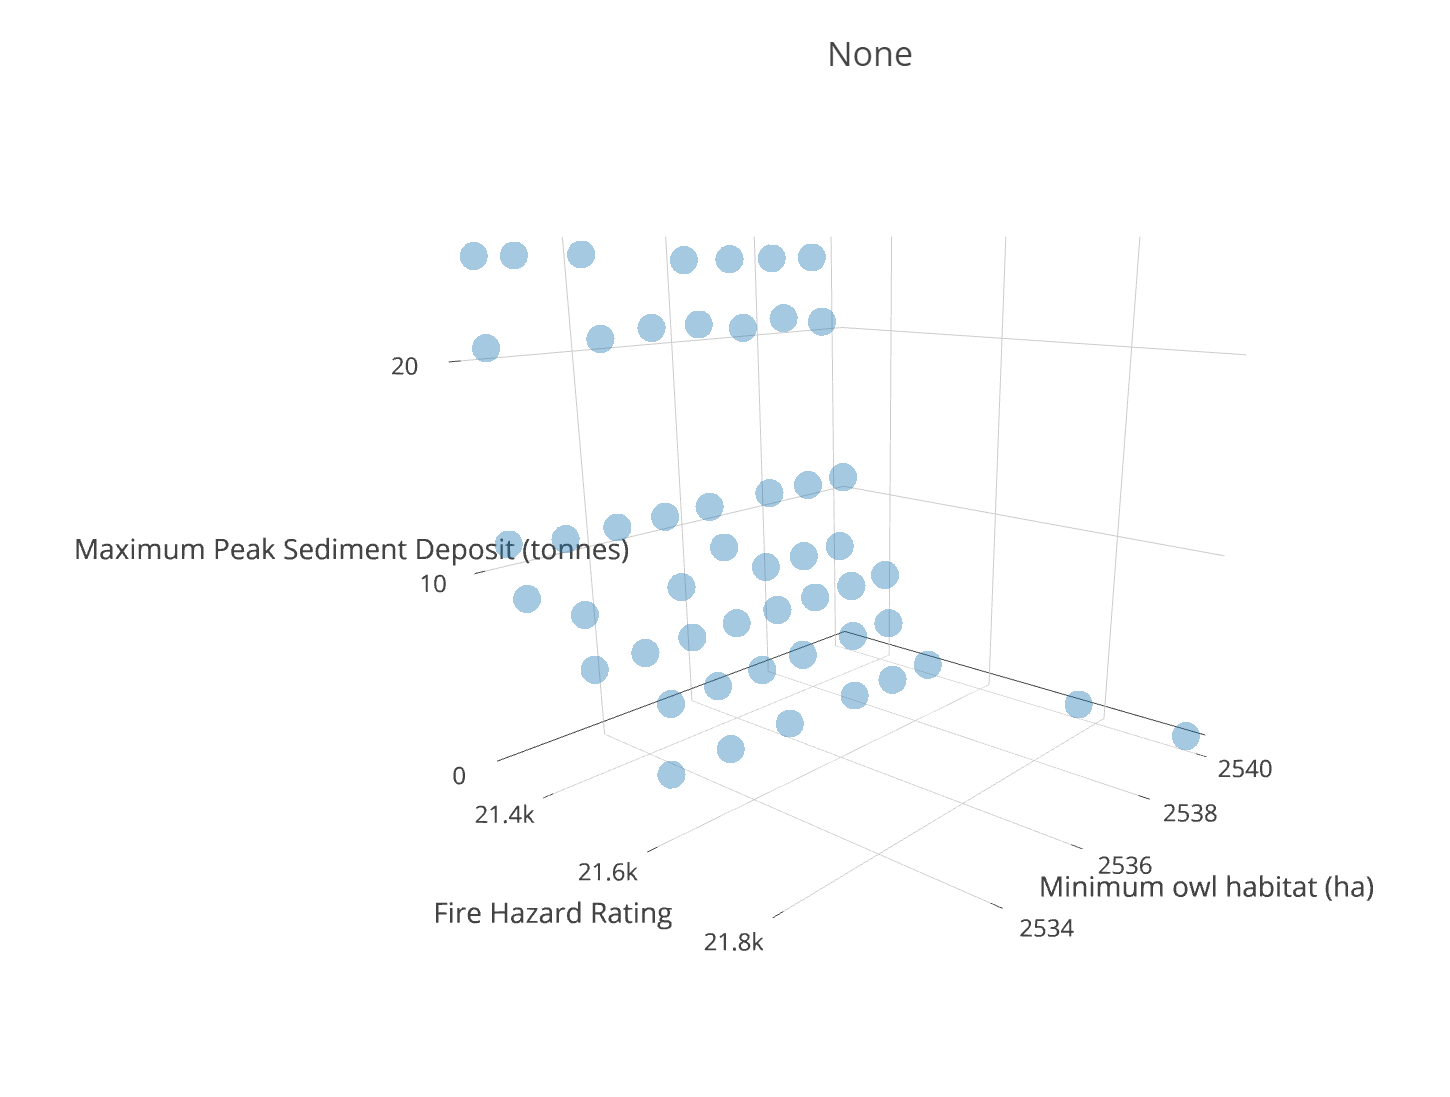
\includegraphics[width=.45\textwidth]{../images/Frontier_None}%
    \label{fig:frontierNone}%
  }
  \subfloat[Ensemble RCP 4.5]{%
    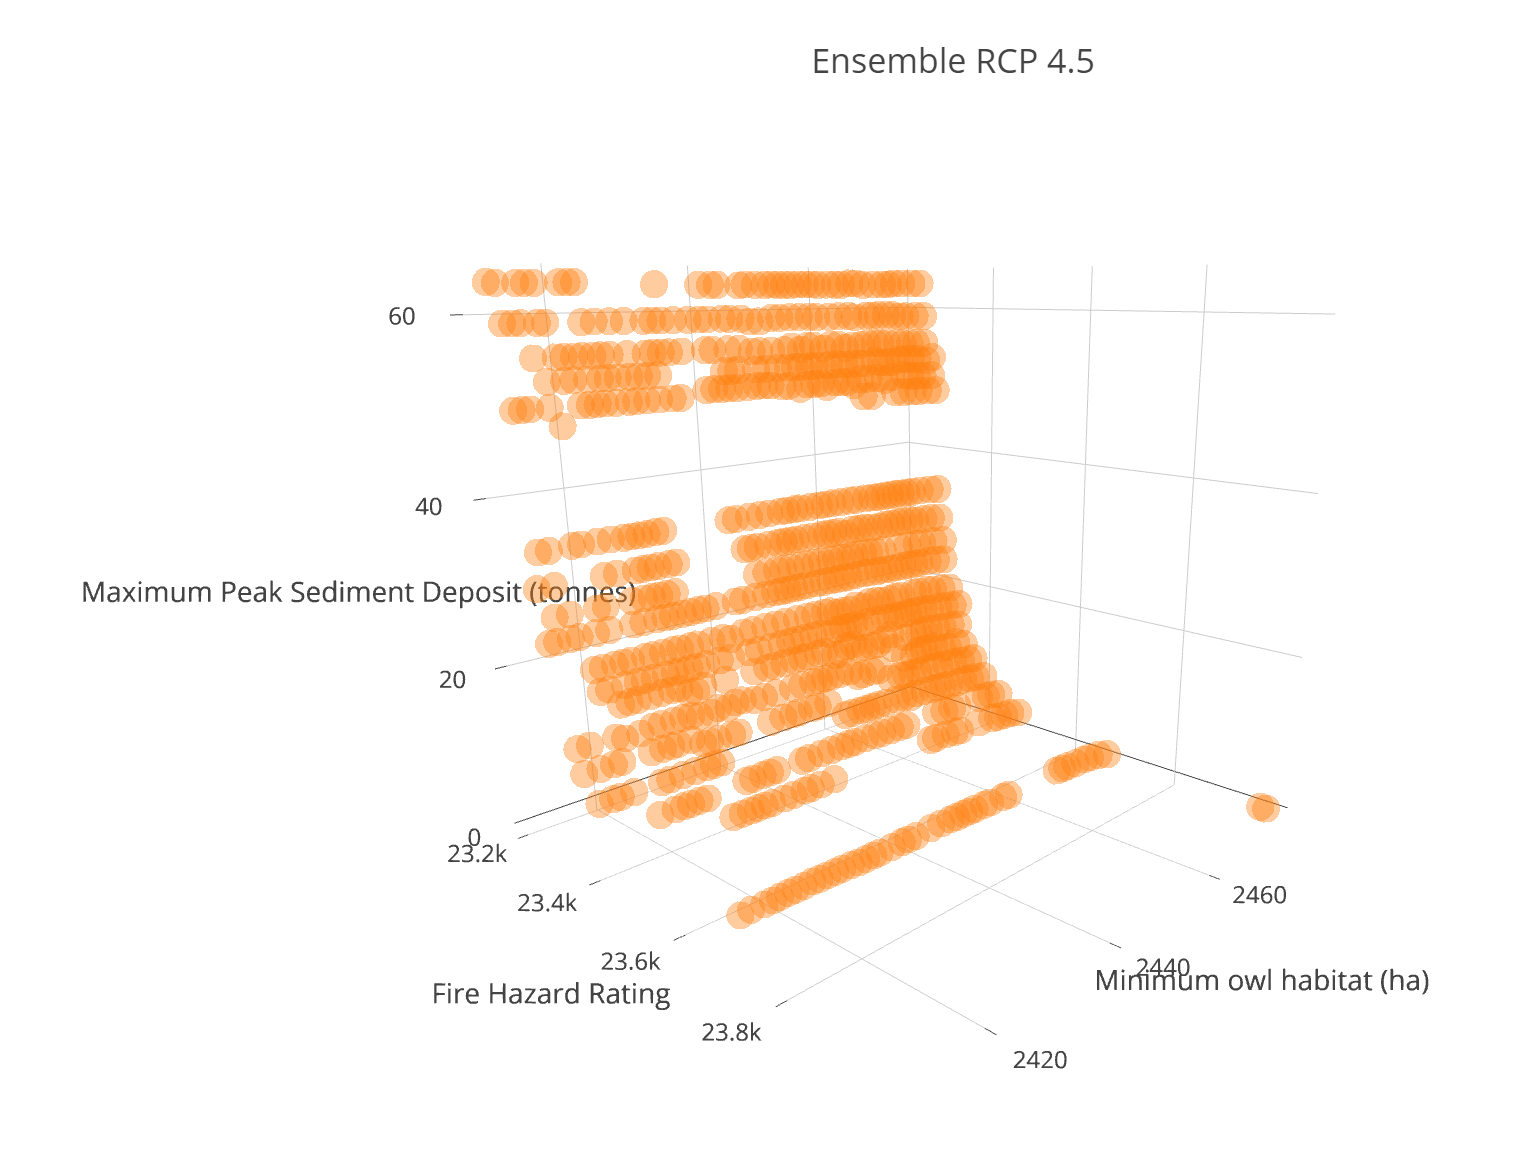
\includegraphics[width=.45\textwidth]{../images/Frontier_E45}%
    \label{fig:frontierE45}%
  }\hfill\centering
  \subfloat[Ensemble RCP 8.5]{%
    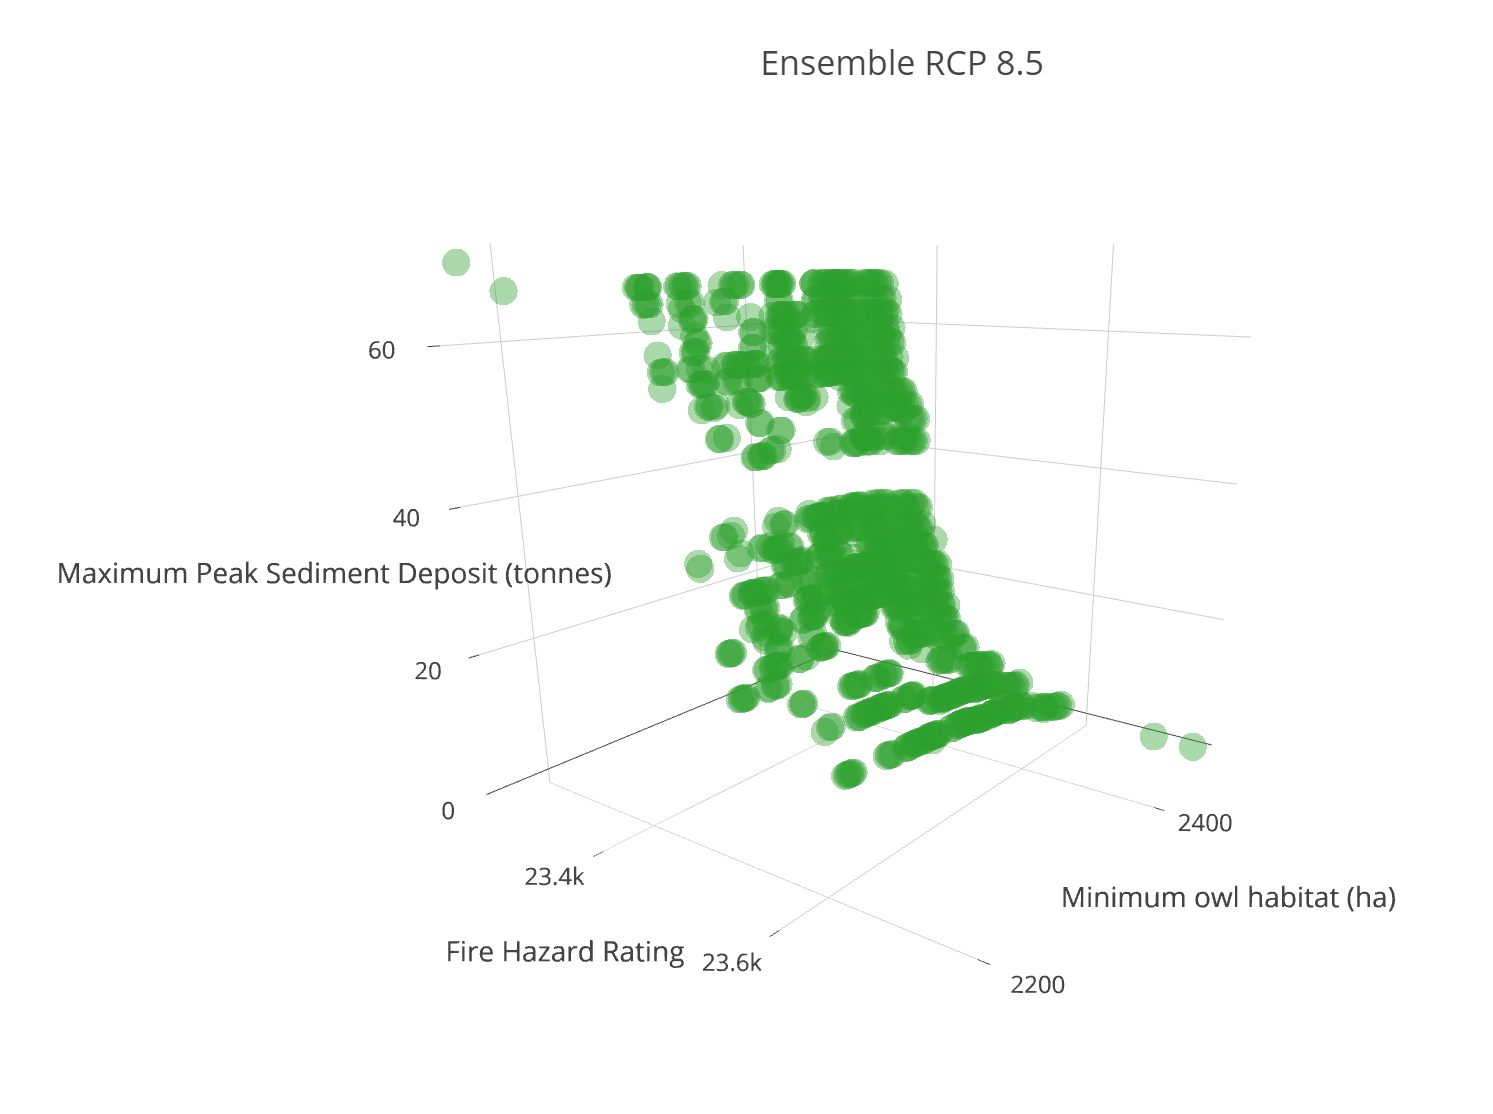
\includegraphics[width=.45\textwidth]{../images/Frontier_E85}%
    \label{fig:frontierE85}%
  }
  \caption[Frontiers for each climate change scenario]{Efficient frontiers for each climate change scenario.}
  \label{fig:frontiersAll}
\end{figure}

\begin{figure}[ht]
\centering
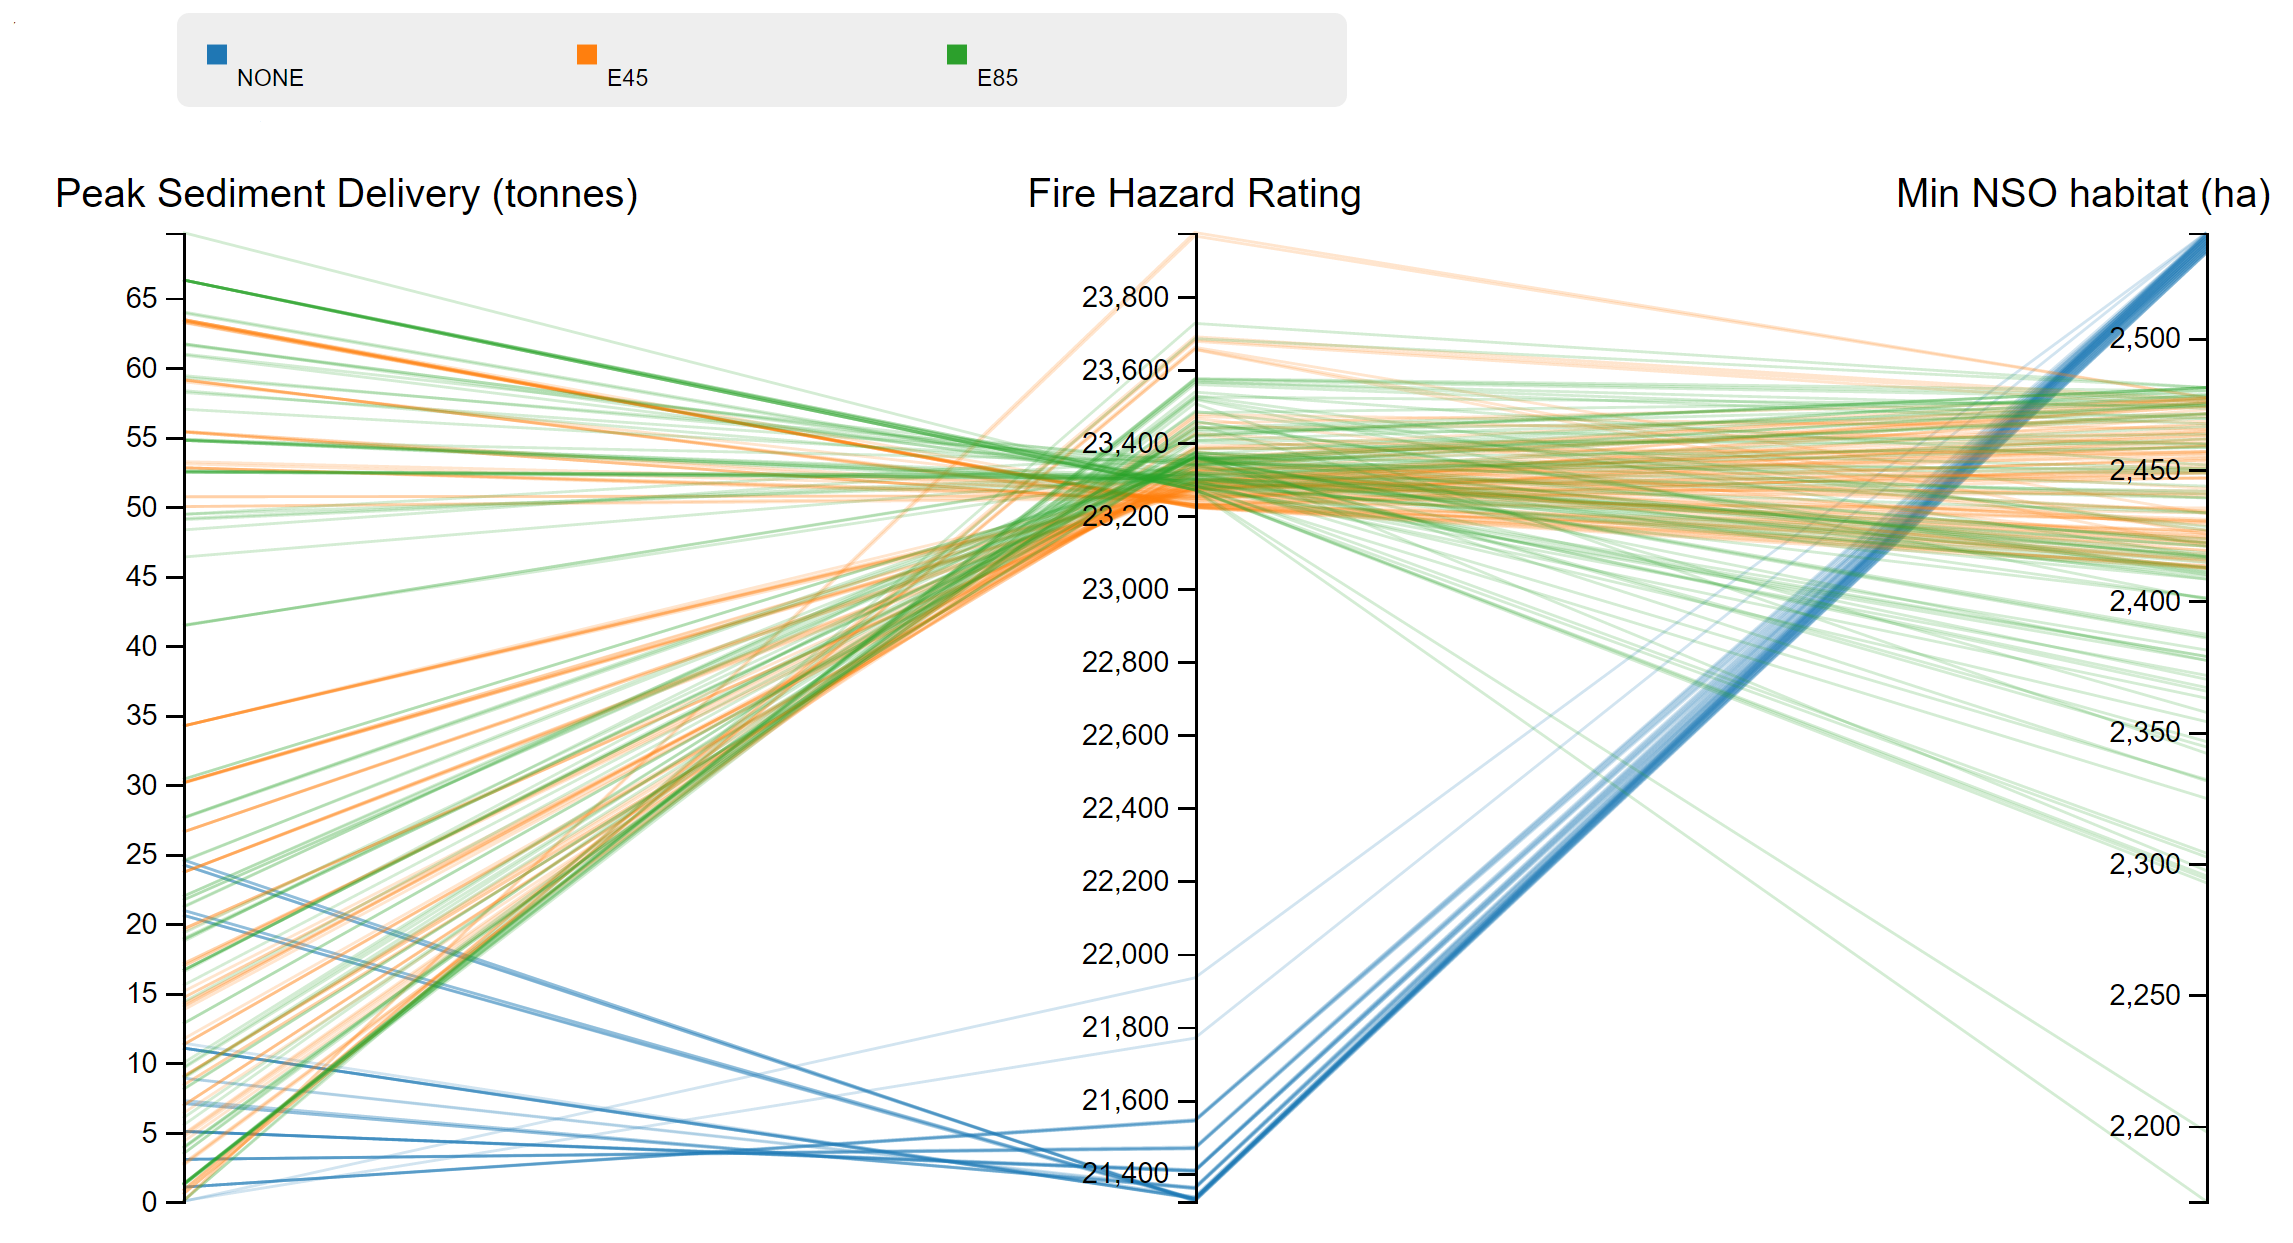
\includegraphics[width=.85\textwidth]{../images/FrontiersPCPlot}
\caption[Parallel coordinates view of the three frontiers]{Parallel coordinates view of the frontiers. Each axis represents an ecosystem service optimized by the model and each line a solution. In all objectives, we notice that None appears to outperform both the E45 and E85 scenarios, which show similar average objective achievements. To increase visual clarity, only a subset of solutions for E45 and E85 are shown because of the number of solutions in these frontiers.}
\label{fig:frontiersPCPlot}
\end{figure}

We begin our analysis by investigating the impacts of climate change on the provision of individual ecosystem services. We then consider how climate change impacts the joint provision of ecosystem services and the conflict among them.

\subsubsection{Provision of individual ecosystem services}
The average achievement of all ecosystem services decreases with increasing severity of climate change (see Table \ref{tab:frontiersSummary}, ``avg'' rows). We find that the difference in ecosystem service provision is greater between the assumption of no climate change and mild climate change (None to E45) than it is between mild climate change and severe climate change (E45 to E85). This suggests that, for the ecosystem services in this study, the realization of climate change is more significant than the severity of that change. The model data provide evidence of why this is the case.

\paragraph{Sediment delivery} 
Compared to the None scenario, the average amount of sediment delivered is 172\% higher in E45 and 204\% higher in E85. To understand why this may be, consider Figure \ref{fig:avgSedimentDelivery}. The figure shows the average tonnes of sediment delivered as a result of performing fuel removals for each climate change scenario. The sediment delivery per fuel removal under E45 is nearly twice the sediment delivery under the None scenario (81\% higher), whereas the E85 scenario is only 0.4\% higher than the E45 scenario.

This is a result of the response in sediment delivery to prescribed burns and the frequency with which they are assigned\footnote{For additional information on how stands are assigned a specific fuel removal technique such as thinning or prescribed burn, see the appendix, \S \ref{chap:appendix_drinkTreatments}.}. Our simulations show that increasing the severity of climate change causes pronounced increases in sediment delivery as a result of prescribed burns. We also find that relative to the None scenario, prescribed burns are assigned more frequently in the climate change scenarios: 8 times more frequently in E45 and 10.1 times more frequently in E85. See Table \ref{tab:prscBurnsInClimChange}. These effects combine to produce the result seen in Figure \ref{fig:avgSedimentDelivery} of increasing sediment levels with climate change severity.

\begin{figure}[ht]
\centering
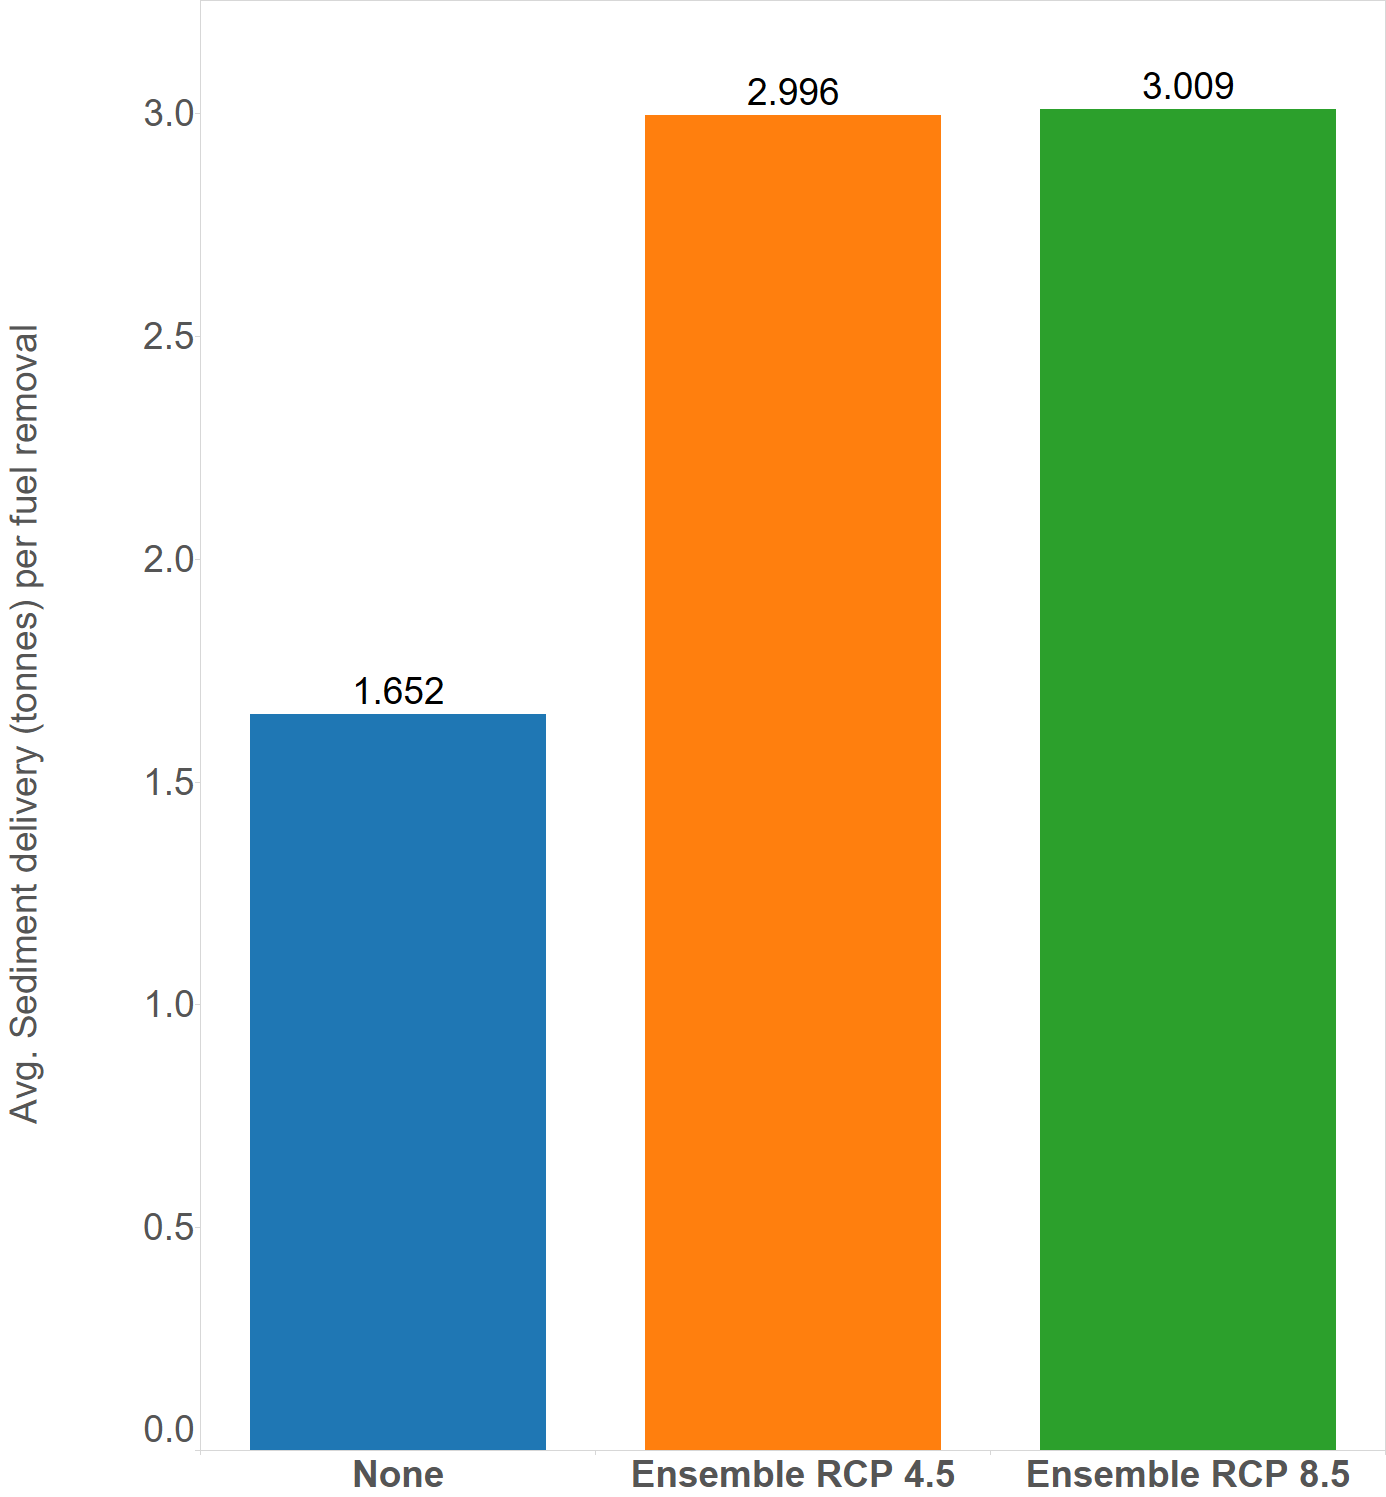
\includegraphics[width=.55\textwidth]{../images/AvgSedimentSpikes}
\caption[Average sediment delivery across climate scenarios]{Average spike in sediment delivery as a result of performing fuel removals for each of the climate change scenarios.}
\label{fig:avgSedimentDelivery}
\end{figure}

\begin{table}[]
\centering
\caption[Frequency and impact of prescribed burns for each climate scenario]{Frequency and impact of prescribed burn for each climate scenario. The combination of more frequent prescribed burns and increased sediment delivery per prescribed burn results in the higher values of sediment delivery in E45 and E85 observed in Figure \ref{fig:avgSedimentDelivery}.}
\label{tab:prscBurnsInClimChange}
\begin{tabular}{l|lll}
                                                                                                           & \textbf{None} & \textbf{E45} & \textbf{E85} \\ \hline
\textbf{\begin{tabular}[c]{@{}l@{}}Average sediment delivery\\ (tonnes) from prescribed burn\end{tabular}} & 31.23            & 48.56          & 48.97          \\
\textbf{\begin{tabular}[c]{@{}l@{}}Number of prescribed\\ burns assigned\end{tabular}}                     & 34         & 272        & 344       
\end{tabular}
\end{table}

\paragraph{Fire hazard}
Similarly, we find that the average fire hazard of the Drink Area increases with climate change severity, with E45 and E85 both performing approximately 9\% worse than None. First, we note that this is not due to the model simply selecting less area for treatment under the climate change scenarios, as this value is essentially constant across both treatment periods and all climate scenarios (see Table \ref{tab:treatedAreas}). Instead, we find that the increase in fire hazard is due to the impact of climate change on the fuel model classification of the stands in the Drink Area. In E45 and E85, more stands are assigned a fuel model classification that is associated with higher fire hazard (refer to table \ref{tab:firehazards} for the mapping from fuel model to fire hazard). This is shown in Figure \ref{fig:distOfFireHazards}, where we observe a larger percentage of stands having a fire hazard rating of either 4 or 5 under the E45 and E85 scenarios than in None.

\begin{table}[]
\centering
\caption[Area treated per period across climate scenarios]{Areas treated per period across climate scenarios. The values are nearly the same for both periods and for each climate scenario.}
\label{tab:treatedAreas}
\begin{tabular}{l|lll}
                                                                                                           & \textbf{None} & \textbf{E45} & \textbf{E85} \\ \hline
\textbf{Area treated (ha) in period 1} & 2427.31            & 2426.90 & 2414.58          \\
\textbf{Area treated (ha) in period 2}                     & 2427.56         & 2427.71        & 2427.63      
\end{tabular}
\end{table}

\begin{figure}[ht]
\centering
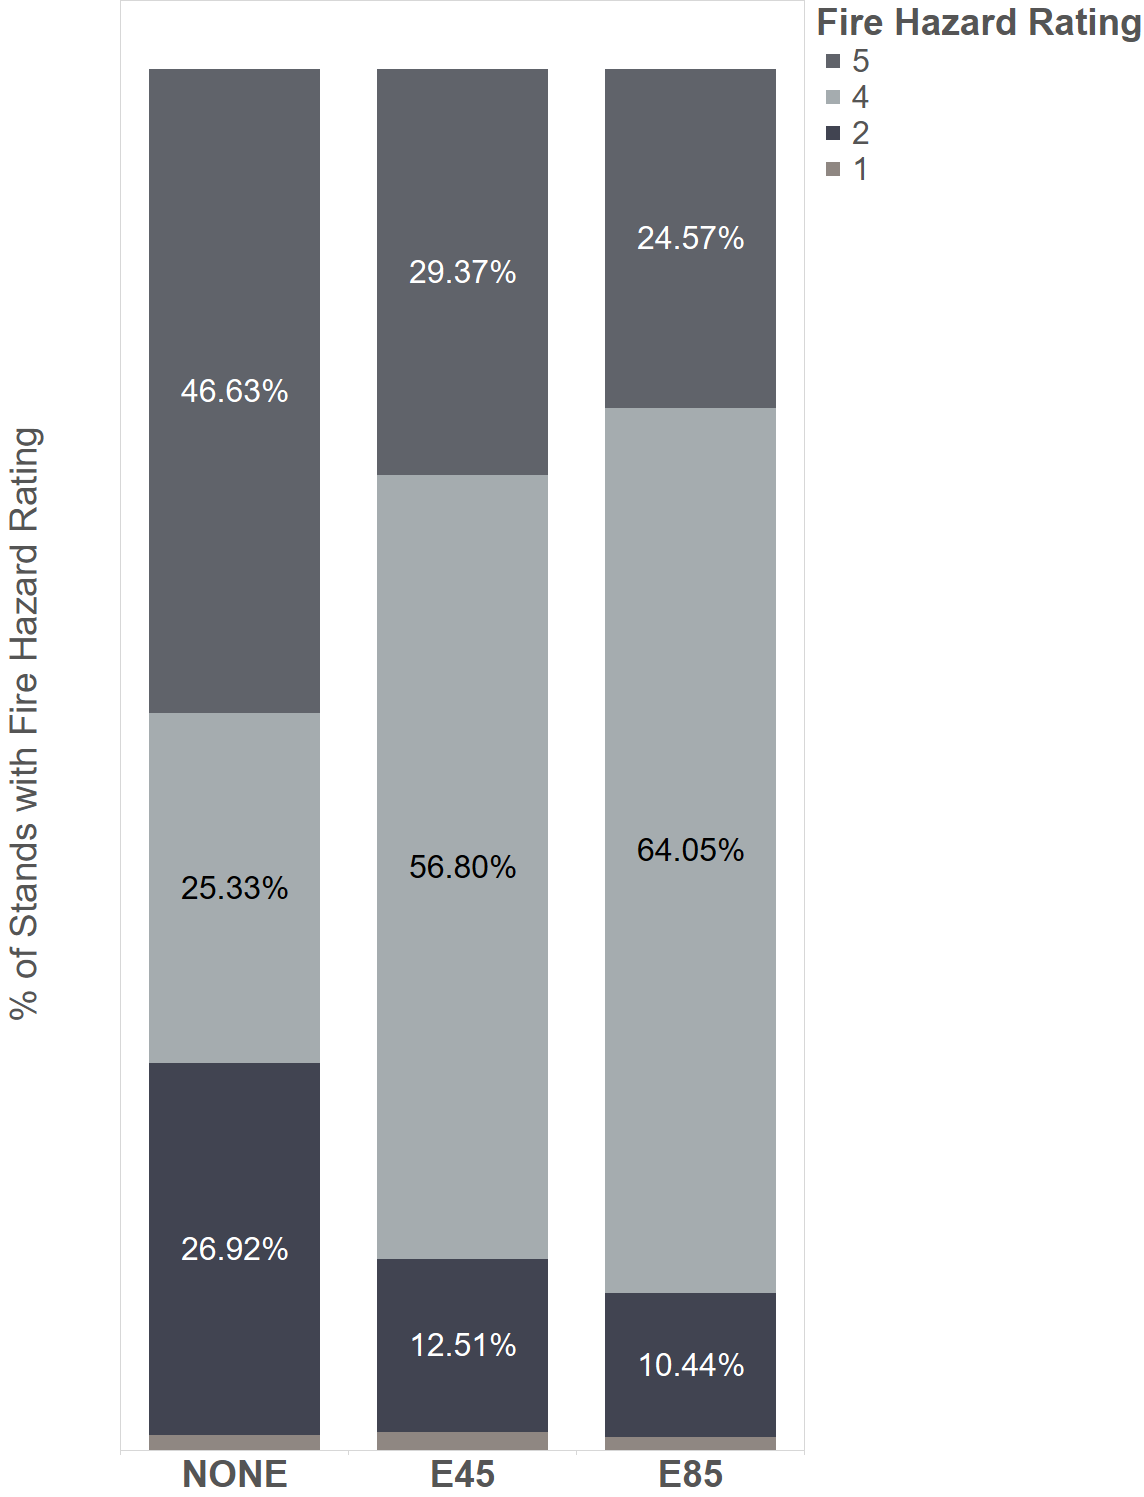
\includegraphics[width=.5\textwidth]{../images/FireHazardRatingsPerClimateScenario}
\caption[Distribution of fire hazard ratings over the Drink Area for each climate change scenario]{Distributions of fire hazard ratings across the Drink Area under each climate change scenario. Moving from left to right (in increasing climate change severity), we observe an increase in the number of stands classified with more extreme fire hazards (ratings of 4 and 5).}
\label{fig:distOfFireHazards}
\end{figure}

\paragraph{NSO habitat}
Finally, we also observe a decrease in the average provision of NSO habitat under the consideration of climate change. The average provision in the E45 scenario is 88.4 ha less than in None, and E85 is 114.3 ha less. The result is likely due to the effects of climate change on the vegetation characteristics that define whether a stand qualifies as NSO habitat. Of the criteria used, two of them are determined by vegetation characteristics: the presence of at least one tree with DBH $> 76$ cm and canopy closure of at least 60\%. While climate change has minimal impact on the former, the average canopy closure for stands in the Drink Area decreases with increasing severity of climate change. See Figure \ref{fig:canopyClosure}.

\begin{figure}[ht]
\centering
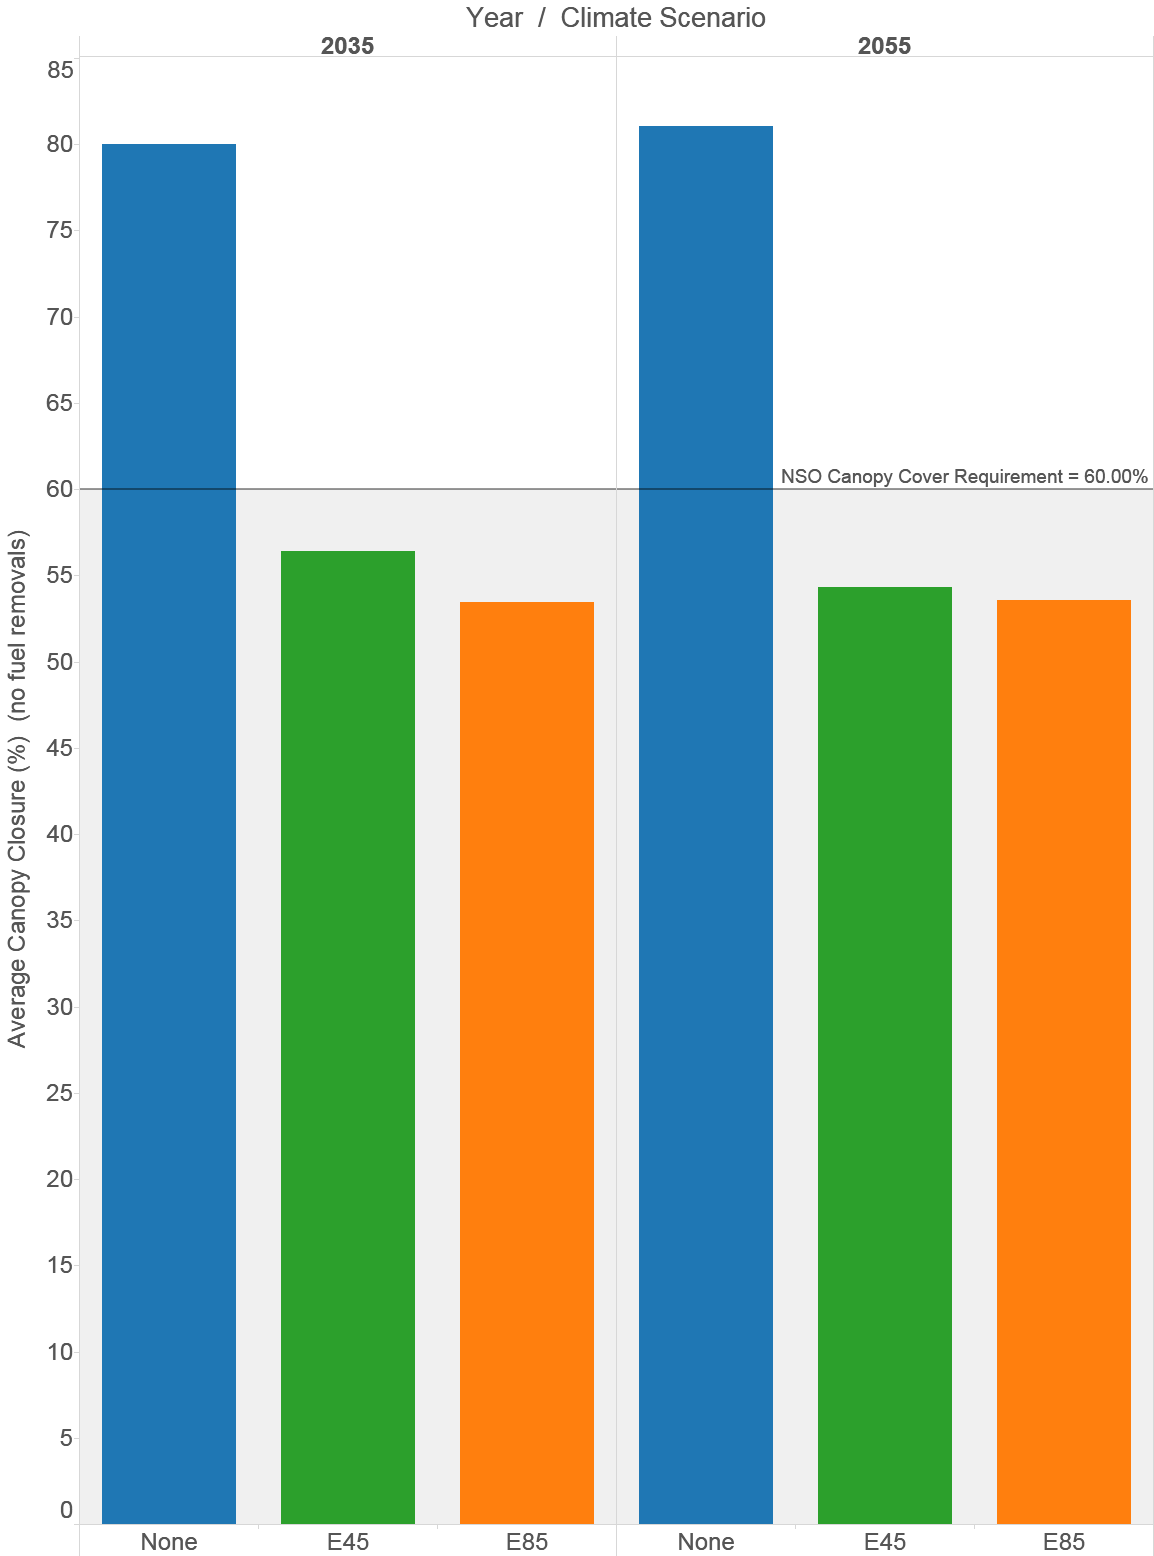
\includegraphics[width=.5\textwidth]{../images/AvgCanopyCover_NoTrtmts}
\caption[Average canopy closure in the Drink Area across climate scenarios]{Average canopy closure for stands in the Drink Area for each climate scenario. Shown are canopy closure values during years 2035 and 2055 (the years in which NSO habitat is measured) when no fuel removals are performed. We see that with increasing climate change severity, canopy closure decreases.}
\label{fig:canopyClosure}
\end{figure}

We also find that the range of achievable values of NSO habitat is small for all climate scenarios, but that the size of this range increases with climate change severity. There are two primary drivers for this increase. The first is in the impact of fuel removals on the amount of NSO habitat available. We see in Table \ref{tab:nsoHabDQs} the number of instances in which performing a fuel removal disqualifies a stand from being NSO habitat under each climate change scenario. This happens more than twice as frequently in E45 and E85 than in None. We also find that the given efficacy in fire hazard reduction when performing a fuel removal that disqualifies a stand from being NSO habitat increases with climate severity. That is, the model is more incentivized to sacrifice NSO habitat in favor of fire hazard reduction. This in turn leads to a reduction in clustering of NSO habitat, further reducing the objective function value (equation NSOOBJVALEQN). This data is shown in Figure MAKEFHEFFECTIVENESSFIG, in which we see the reduction in fire hazard as a result of fuel removals that disqualify a stand as NSO habitat. We see that these values increase with climate change severity.

% USE THIS IN THE CONFLICT SECTION FOR NSO VS FIRE HAZARD
\begin{table}[ht]
\centering
\caption[Frequency of NSO habitat disqualifications for each climate scenario]{Shown here are the number of times for each climate scenario that a fuel removal triggers the disqualification of a stand from being NSO habitat.}
\label{tab:nsoHabDQs}
\begin{tabular}{l|l}
\textbf{Climate change scenario} & \begin{tabular}{@{}l@{}}\textbf{Disqualifications of NSO habitat} \\ \textbf{as a result of fuel removals}\end{tabular} \\ \hline
\textbf{None}                    & 24                                                                               \\
\textbf{Ensemble RCP 4.5}        & 60                                                                               \\
\textbf{Ensemble RCP 8.5}        & 60                                                                              
\end{tabular}
\end{table}

in part due to the impact of fuel removals on due to the impact of the aforementioned vegetation changes on the ability of NSO habitat to form in clusters.

\subsubsection{Joint provision of ecosystem services}
Our results show that climate change will also have an impact on the joint provision of ecosystem services. We observe a decreasing hypervolume with increasing severity of climate change - see Table \ref{tab:hypervols}. A decreasing hypervolume is indicative of more conflict in the system, meaning that climate change is associated with more conflict among the ecosystem services.

\begin{table}[]
\centering
\caption[Hypervolumes of the efficient frontiers]{Hypervolume for each climate change scenario. Hypervolume values increase with increasing severity of climate change.}
\label{tab:hypervols}
\begin{tabular}{lllll}
\multicolumn{2}{l|}{}                                                  & \textbf{None} & \textbf{E45} & \textbf{E85} \\ \hline
\multicolumn{2}{l|}{\textbf{Hypervolume}}                              & 0.876977      & 0.866857     & 0.829541       
\end{tabular}
\end{table}

The difference in hypervolume between None and E45 is approximately 0.01. Recall that a difference of $h$ in hypervolumes equates to a difference of $h^{1/M}$ in each objective. Thus, despite the small size of the difference between $I_{H1}(Z_\text{None})$ and $I_{H1}(Z_\text{E45})$, it signifies an additional achievement in each objective of approximately 21.6\%. The difference is greater between None and E85, approximately 0.05, which represents an additional achievement in each objective of 36.2\%.

From the hypervolumes alone, it is uncertain whether None represents a strictly better frontier than either E45 or E85 or if, despite their smaller hypervolume values, E45 and E85 enclose some region of the objective space that is not enclosed by None. We use the binary hypervolume indicator $I_{H2}$ to address this question.

The binary hypervolume values for each pair of frontiers are shown in Table \ref{tab:binaryHypervols}. The binary hypervolume values tend to align with the hypervolume values, with larger binary hypervolumes when $I_{H1}(Z_1) > I_{H1}(Z_2)$ and smaller values when $I_{H1}(Z_2) > I_{H1}(Z_1)$. Interestingly, all binary hypervolume values are positive, indicating that no frontier is dominated by any other; each frontier uniquely encloses some region of the objective space. This region of the objective space bound only by a frontier $Z_i$ indicates the presence solutions in climate scenario $i$ that achieve greater joint provision of ecosystem services.% than those in the other climate scenarios in this region. 

\begin{table}[]
\centering
\caption[Binary hypervolume values for each pair of climate scenarios]{Binary hypervolumes for each pair of climate scenarios. No values are negative, indicating that no frontiers are dominated by another and that all frontiers uniquely enclose some volume of the objective space.}
\label{tab:binaryHypervols}
\begin{tabular}{ll|l}
\textbf{$Z_1$} & \textbf{$Z_2$} & \textbf{$I_{H2}(Z_1,Z_2)$} \\ \hline
\textbf{None}  & \textbf{E45}   & 0.026154                   \\
\textbf{None}  & \textbf{E85}   & 0.058001                   \\
\textbf{E45}   & \textbf{None}  & 0.016034                   \\
\textbf{E45}   & \textbf{E85}   & 0.045156                   \\
\textbf{E85}   & \textbf{None}  & 0.010565                   \\
\textbf{E85}   & \textbf{E45}   & 0.007841                  
\end{tabular}
\end{table}

To determine the location of these regions and better understand the basis of the change in conflict between climate scenarios, we examine pairwise objective relationships.

\paragraph{Sediment delivery-NSO Habitat}
We observe no clear relationship between climate change severity and the conflict between sediment delivery and NSO habitat; see Figure \ref{fig:pairplotNSOSed}. The figure shows the efficient frontier plotted in the sediment delivery-NSO habitat plane, where each objective has been normalized such that better values are higher and worse values are lower. For instance, in this graph, the point $(1,1)$ represents 0 sediment delivery and maximum NSO habitat. We see similar uniform spreads of solutions for each climate scenario.

\begin{figure}[ht]
\centering
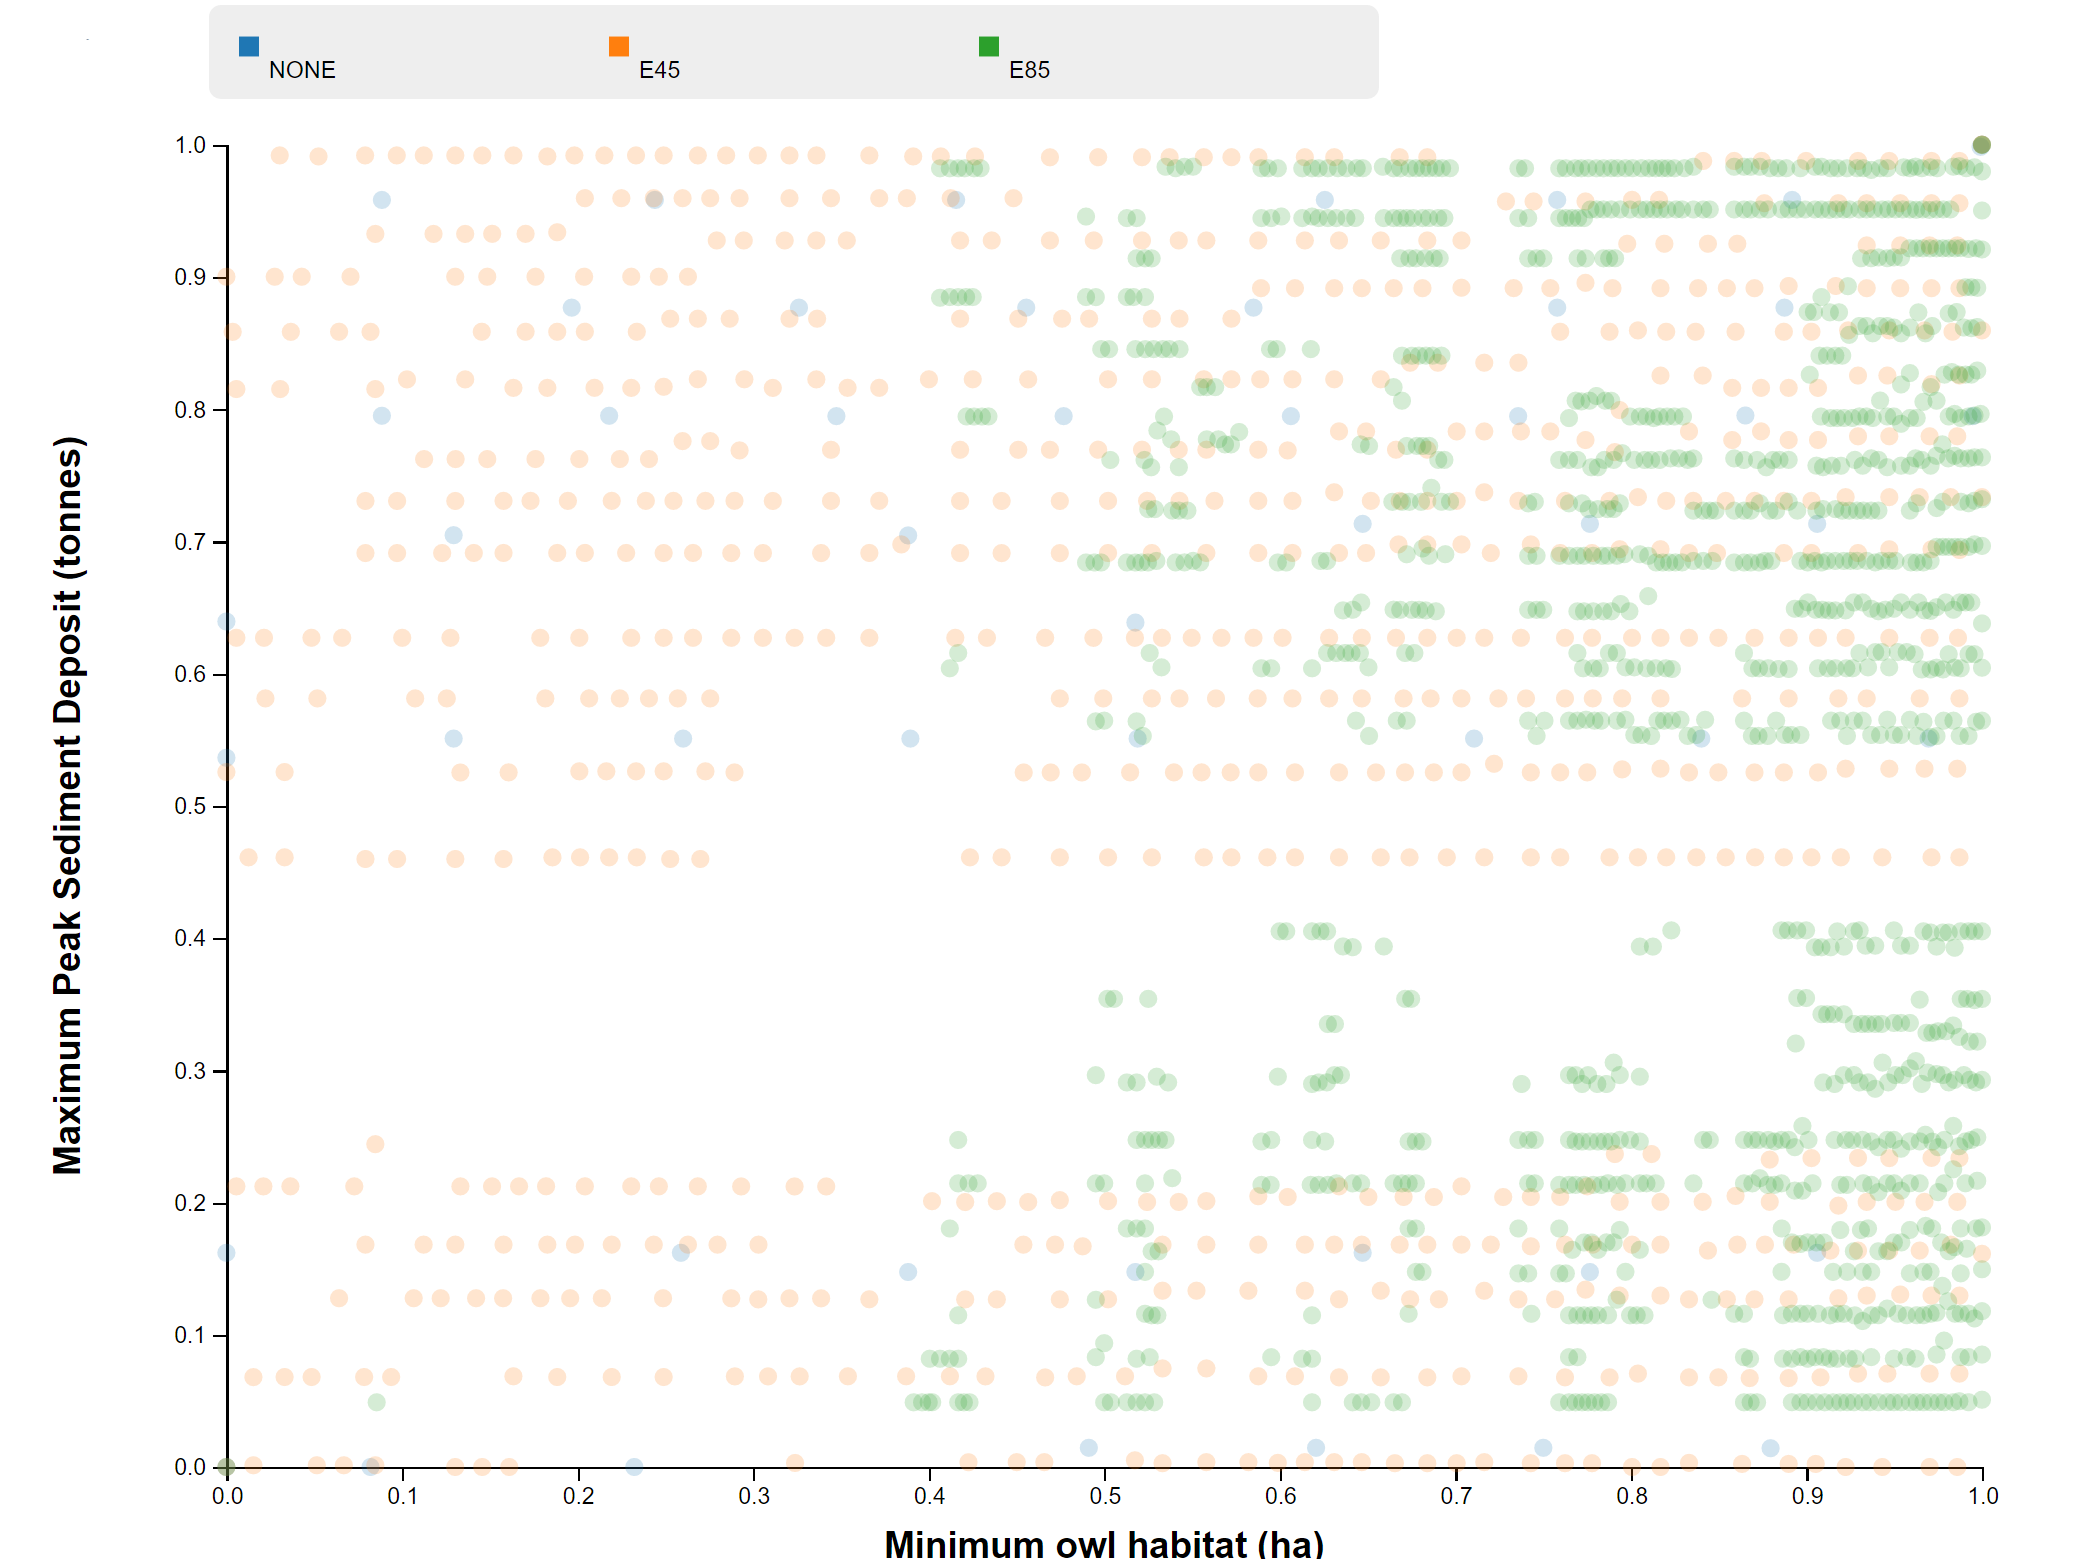
\includegraphics[width=.75\textwidth]{../images/2DSlice_NSO_Sed}
\caption[NSO habitat vs. sediment delivery for all climate scenarios]{NSO habitat versus sediment delivery for all climate scenarios. No obvious conflict pattern exists between the objectives in any climate scenario.}
\label{fig:pairplotNSOSed}
\end{figure}

The values for pairwise conflict also indicate a lack of conflict, as seen in Table \ref{tab:pairConflict-SedNSO}. Values for $C_{ij}$ are all less than $0.25$, with the highest value for the E45 scenario and lower values for E85 and None. To determine the reason for the variation in $C_{ij}$ by climate scenario, we disassemble the conflict metric into components. A value of $c_{ij,\rho} = 0.5$ indicates the absence of rank correlation, and we find no climate scenario that differs significantly from this value. Lower values of $c_{ij,\rho}$ indicate positive rank correlation, such as in None ($c_{ij,\rho}=0$ for non-conflicting objectives); higher values for $c_{ij,\rho}$ indicate more conflict. $c_{ij,d} \in [0,1]$ represents the average distance of solutions from the sub-dimensional ideal solution. The solutions in the E45 and None scenarios are further away from the sub-dimensional ideal solution than those in E85 leading to larger values of $c_{ij,d}$, but all climate scenarios have on average solutions that are near the mid-point mark of $c_{ij,d} = 0.5$.

\begin{table}[]
\centering
\caption[Sediment-NSO conflict across climate scenarios]{Conflict between sediment delivery and NSO habitat across climate scenarios.}
\label{tab:pairConflict-SedNSO}
\begin{tabular}{l|l|ll}
\textbf{}     & \textbf{$C_{ij}$} & \textbf{$c_{ij,\rho}$} & \textbf{$c_{ij,d}$} \\ \hline
\textbf{None} & 0.19639           & 0.3974                 & 0.4942              \\
\textbf{E45}  & 0.25667           & 0.5194                 & 0.4941              \\
\textbf{E85}  & 0.19284           & 0.5160                 & 0.3737             
\end{tabular}
\end{table}

\paragraph{NSO habitat-fire hazard}
According to the conflict metric proposed here, the conflict between NSO habitat and fire hazard is small for all climate scenarios but appears to decrease with increasing severity of climate change. We find this is due primarily to the increasing density of solutions nearer the sub-dimensional ideal solution in the E45 and E85 scenarios compared to None. See Figure ADDIN2DSLICEFIGURE. Breaking the conflict metric again into components (see Table MAKETHECOMPONENTRYTABLE), we see that the average distance to the ideal decreases with increasing severity of climate change, while the rank correlation again does not differ significantly from $0.5$.


% Per stand, avg reduction in fire hazard vs sediment delivered as a result of fuel removal

% For a given fuel removal that disqualifies a stand as NSO habitat, what is the difference in fire hazard between the "NONE" and (whatever that fuel removal action was) is?

\subsection{General results}
\subsubsection{New conflict metric}

\paragraph{Pros}
We saw that fire-sed relationship got worse, and data supported that.

\paragraph{Cons}
When looking at all pairwise conflict metrics for a frontier, their combination does not let you make deductions of the whole system level conflict.
Weights average objective achievement perhaps too much. Frontiers with a bunch of solutions nearer the ideal are given less conflict. perhaps that's OK though.


TO TALK ABOUT SOMEWHERE:
Why the disparity in number of solutions?
Why E85 achieve relatively more NSO habitat and relatively less FH on average than the others (fig \ref{fig:pairplotNSOSed} and sim for NSO-FH)?
The increased range in achievable values for the objs in the case of climate change leads to results that show tighter clustering closer to ideal, which weights the conflict towards "less". Basically, more extreme extremes make most other values seem more normal(?).

INVESTIGATE MORE:
What's the difference in actual acreage of NSO hab vs diffs due to clustering discounts?
NUM SOLUTIONS = bc of the DQing of NSO hab as a result of actions, there are more combos of ways to do that and pvar values as a result.